\documentclass[11pt,letterpaper]{article}
\usepackage[utf8]{inputenc}

%----- Configuración del estilo del documento------%
\usepackage{epsfig,graphicx}
\usepackage[left=2cm,right=2cm,top=1.8cm,bottom=2.3cm]{geometry}
\usepackage{fancyhdr}
\usepackage{lastpage}

\usepackage{xcolor}
\usepackage{soul}
\newcommand{\mathcolorbox}[2]{\colorbox{#1}{$\displaystyle #2$}}

%------ Paquetes para demostraciónes y árboles de derivación ------%
\usepackage{bussproofs}
\usepackage{scalefnt}

%Color bibi
\definecolor{bibi}{RGB}{0,103,148}
% Otros colores

% ------ Paquetes para arboles --------%
\usepackage{bussproofs}

\usepackage{cite}
\usepackage{multicol}
\setlength{\columnsep}{1.5cm}
\setlength{\columnseprule}{.5pt}

\pagestyle{fancy}
\fancyhf{}
\rfoot{\textit{Página \thepage \hspace{1pt} de \pageref{LastPage}}}

%------ Paquetes matemáticos básicos --------%
\usepackage{amsmath}
\usepackage{amssymb}
\usepackage{amsthm}

%------ Paquetes para codigo --------%
\usepackage{verbatim}

\begin{document}
%------ Encabezado -------- %
\begin{center}
    \begin{minipage}{3cm}
    	\begin{center}
    		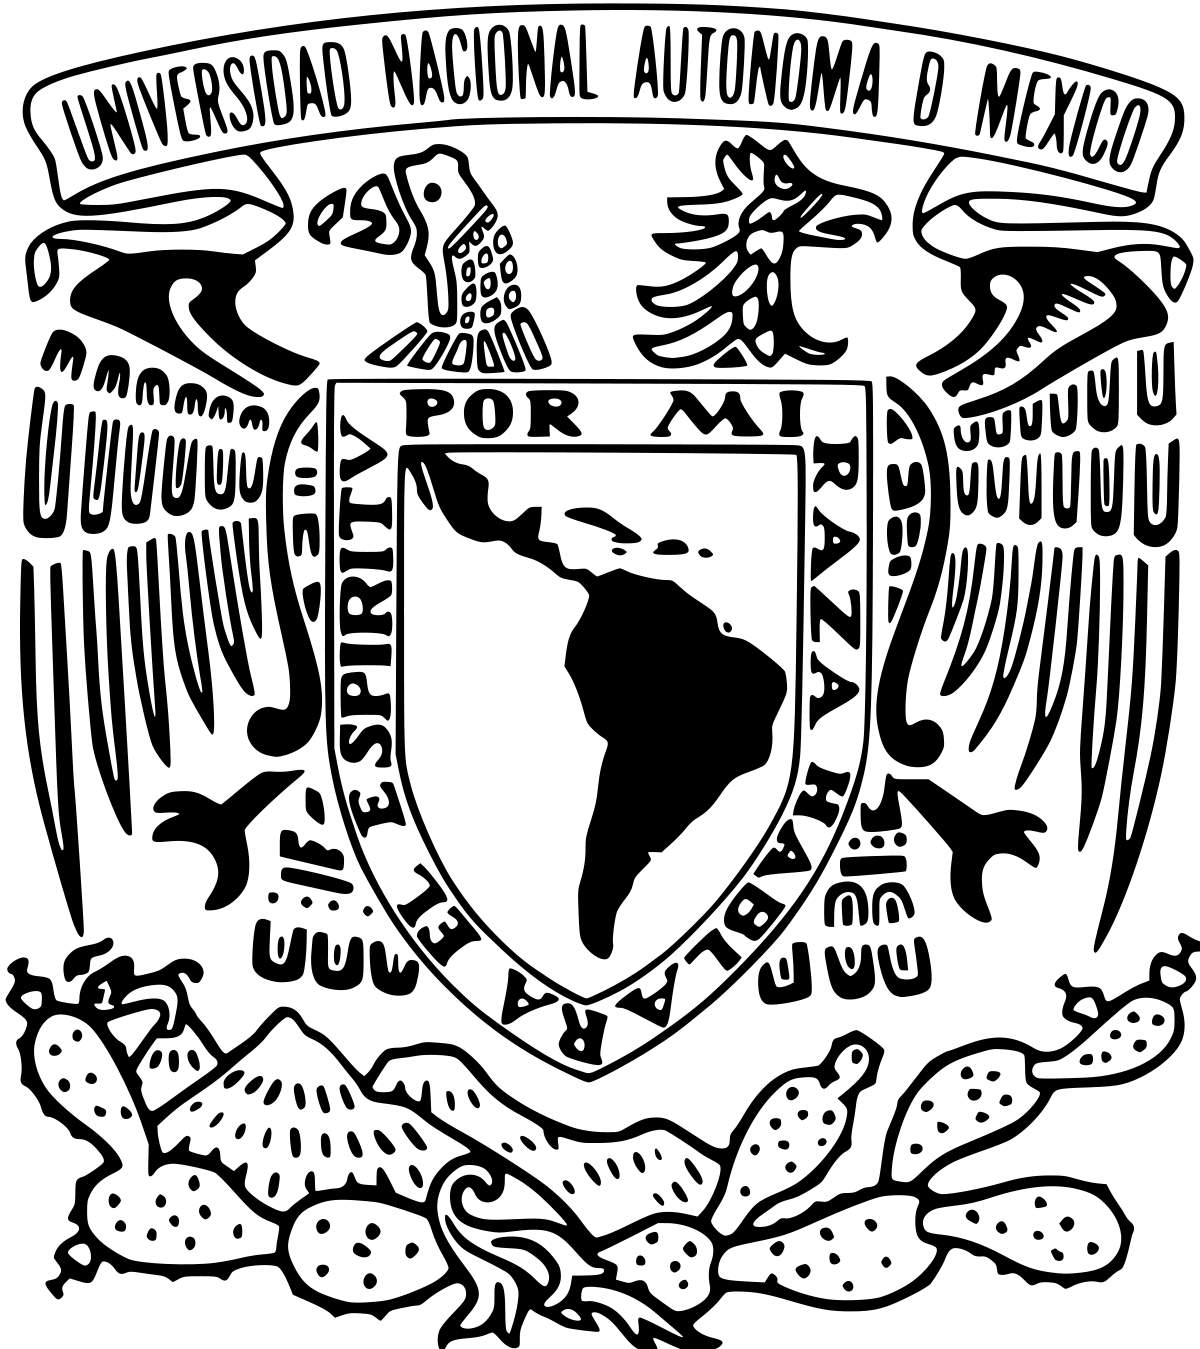
\includegraphics[height=3.4cm]{src/Img/Logo_UNAM.png}
    	\end{center}
    \end{minipage}\hfill
    \begin{minipage}{10cm}
    	\begin{center}
    	\textbf{\large Universidad Nacional Autónoma de México}\\[0.1cm]
        \textbf{Facultad de Ciencias}\\[0.1cm]
        \textbf{Lenguajes de Programación  $|$ 7098}\\[0.1cm]
        Semanal 6 : $|$ Ambientes con diferentes alcances\\[0.1cm]
        Sosa Romo Juan Mario $|$ 320051926 \\[0.1cm]
        Legorreta Esparragoza Juan Luis $|$ 319317532 \\[0.1cm]
        Erik Eduardo Gómez López $|$ 320258211 \\[0.1cm]
        24/09/24
    	\end{center}
    \end{minipage}\hfill
    \begin{minipage}{3cm}
    	\begin{center}
    		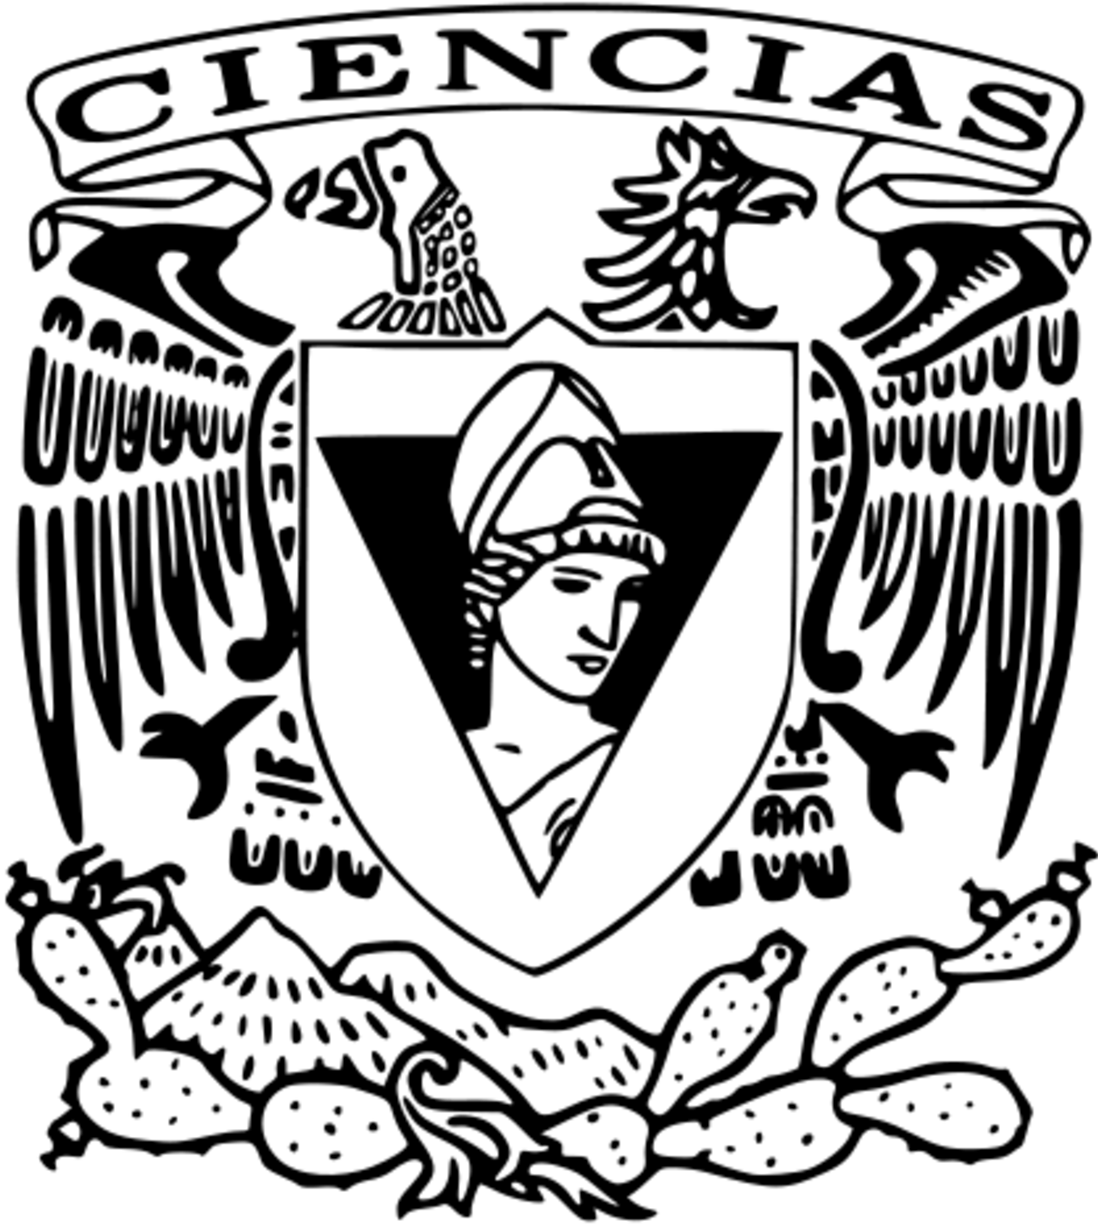
\includegraphics[height=3.4cm]{src/Img/Logo_FC.png}
    	\end{center}
    \end{minipage}
\end{center}


\rule{17cm}{0.1mm}


%------ Ejercicios -------- %
\begin{center}
    \textbf{Evaluar las siguientes expresiones usando a) sustitución, b) ambientes con alcance dinámico y c) ambientes con alcance estático. Es necesario que muestren el ambiente de evaluación final en forma de pila en los casos que corresponda. Para el inciso c) además deberán indicar la cerradura de cada función.}\vspace{.2cm}
    
    \textbf{Nota: }En esta ocasión no será necesario que muestren la sintaxis abstracta de las expresiones
\end{center}
\begin{enumerate}
    \item \begin{verbatim}
    (let (a 2)
        (let (b 3)
            (let (foo (lambda (x) (- (+ a b) x)))
                (let (a -2)
                    (let (b -3)
                        (let (foo (lambda (x) (+ (- a b) x)))
                            (foo - 10)))))))
\end{verbatim}


    \begin{enumerate}
        \item Sustituimos y resolvemos para $a$ y $b$:
\begin{verbatim}
    (let (foo (lambda (x) (- 5 x)))
        (let (a -2)
            (let (b -3)
                (let (foo (lambda (x) (+ (- a b) x)))
                    (foo - 10)))))
\end{verbatim}

Nuevamente sustituimos y resolvemos $(a -2)$ y $(b -3)$ para el siguiente foo:\\
\begin{verbatim}
    (let (foo (lambda (x) (+ (- (-2) (-3) x)))
                    (foo - 10))
\end{verbatim}
Evaluamos:
\begin{verbatim}
    (let (foo (lambda (x) (+ 1 x)))
                    (foo - 10))
\end{verbatim}
El primer $foo$ queda reescrito por el segundo, por lo que lo sustituímos en la expresión final:
\begin{verbatim}
    ((lambda (x) (+ 1 x)) -10)
\end{verbatim}
Evaluamos:
\begin{verbatim}
    (+ 1 -10)
    (-9)
\end{verbatim}
El resultado final es igual a -9.

        \item \textbf{Comenzamos construyendo el ambiente y se queda el cuerpo:}

\vspace{.3cm}

\textbf{Pila:}
\[
\begin{array}{c}
  foo \Leftarrow (lambda (x) (- (+ a b) x))\\
  b \Leftarrow 3 \\
  a \Leftarrow 2 \\
\end{array}
\]

\textbf{Nos queda:}
\begin{verbatim}
(let (a -2)
    (let (b -3)
        (let (foo (lambda (x) (+ (- a b) x)))
            (foo -10))))
\end{verbatim}

Volvemos a agregar los siguientes valores a la pila:

\vspace{.3cm}
\[
\begin{array}{c}
  foo \Leftarrow (lambda (x) (- (+ a b) x))\\
  b \Leftarrow -3 \\
  a \Leftarrow -2 \\
  foo \Leftarrow (lambda (x) (- (+ a b) x))\\
  b \Leftarrow 3 \\
  a \Leftarrow 2 \\
\end{array}
\]

\textbf{Nos queda:}
\begin{verbatim}
    (foo -10)
\end{verbatim}

\textbf{Evaluamos, buscamos el valor de \texttt{foo} en la pila,}

\vspace{.3cm}

\textbf{Nos queda:}
\begin{verbatim}
((lambda (x) (+ (- a b) x)) -10)
\end{verbatim}

Agregamos el valor de $x$ a la pila:
\[
\begin{array}{c}
  x \Leftarrow -10\\
  foo \Leftarrow (lambda (x) (- (+ a b) x))\\
  b \Leftarrow -3 \\
  a \Leftarrow -2 \\
  foo \Leftarrow (lambda (x) (- (+ a b) x))\\
  b \Leftarrow 3 \\
  a \Leftarrow 2 \\
\end{array}
\]

\textbf{Nos queda:}
\begin{verbatim}
(+ (- a b) x)
\end{verbatim}

\textbf{Buscamos los valores de \texttt{a}, \texttt{b} y \texttt{x} en la pila:}

\vspace{.3cm}

\textbf{Nos queda:}
\begin{verbatim}
(+ (- (-2) (-3)) -10)
\end{verbatim}

\textbf{Resolvemos la operación:}

\[
(- (-2) (-3)) = 1
\]

\textbf{Nos queda:}
\begin{verbatim}
(+ 1 -10)
(-9)
\end{verbatim}

El resultado final es -9.

        \item Comenzamos construyendo el ambiente y se queda el cuerpo: \vspace{.3cm}

\textbf{Pila:}
\[
\begin{array}{c}
  a \Leftarrow 2
\end{array}
\]

\textbf{Nos queda:}
\begin{verbatim}
    (let (b 3)
        (let (foo (lambda (x) (- (+ a b) x)))
            (let (a -2)
                (let (b -3)
                    (let (foo (lambda (x) (+ (- a b) x)))
                        (foo - 10))))))
\end{verbatim}

Repetimos, metemos a b en la pila y seguimos con el cuerpo: \vspace{.3cm}

\textbf{Pila:}
\[
\begin{array}{c}
    b \Leftarrow 3 \\
    a \Leftarrow 2
\end{array}
\]

\textbf{Nos queda:}
\begin{verbatim}
    (let (foo (lambda (x) (- (+ a b) x)))
        (let (a -2)
            (let (b -3)
                (let (foo (lambda (x) (+ (- a b) x)))
                    (foo - 10)))))
\end{verbatim}

Repetimos, metemos foo en la pila y seguimos con el cuerpo (ojo que aqui
vamos a tener que crear una segunda pila que sera el ambiente de foo): \vspace{.3cm}

\textbf{Pila:}
\[
\begin{array}{c}
    foo \Leftarrow <x,(- (+ a b) x),\varepsilon_1> \\
    b \Leftarrow 3 \\
    a \Leftarrow 2
\end{array}
\]

\textbf{Pila $\varepsilon_1$:} (ambiente de foo)
\[
\begin{array}{c}
    b \Leftarrow 3 \\
    a \Leftarrow 2
\end{array}
\]

\textbf{Nos queda:}
\begin{verbatim}
    (let (a -2)
        (let (b -3)
            (let (foo (lambda (x) (+ (- a b) x)))
                (foo - 10))))
\end{verbatim}

Repetimos, metemos a en la pila y seguimos con el cuerpo: \vspace{.3cm}

\textbf{Pila:}
\[
\begin{array}{c}
    a \Leftarrow -2 \\
    foo \Leftarrow <x,(- (+ a b) x),\varepsilon_1> \\
    b \Leftarrow 3 \\
    a \Leftarrow 2
\end{array}
\]

\textbf{Pila $\varepsilon_1$:} (ambiente de foo)
\[
\begin{array}{c}
    b \Leftarrow 3 \\
    a \Leftarrow 2
\end{array}
\]

\textbf{Nos queda:}
\begin{verbatim}
    (let (b -3)
        (let (foo (lambda (x) (+ (- a b) x)))
            (foo - 10)))
\end{verbatim}

Repetimos, metemos b en la pila y seguimos con el cuerpo: \vspace{.3cm}

\textbf{Pila:}
\[
\begin{array}{c}
    b \Leftarrow -3 \\
    a \Leftarrow -2 \\
    foo \Leftarrow <x,(- (+ a b) x),\varepsilon_1> \\
    b \Leftarrow 3 \\
    a \Leftarrow 2
\end{array}
\]

\textbf{Pila $\varepsilon_1$:} (ambiente de foo)
\[
\begin{array}{c}
    b \Leftarrow 3 \\
    a \Leftarrow 2
\end{array}
\]

\textbf{Nos queda:}
\begin{verbatim}
    (let (foo (lambda (x) (+ (- a b) x)))
        (foo - 10))
\end{verbatim}

Repetimos, metemos foo en la pila y seguimos con el cuerpo (ojo que aqui
vamos a tener que crear una segunda pila que sera el ambiente de foo): \vspace{.3cm}

\textbf{Pila:}
\[
\begin{array}{c}
    foo \Leftarrow <x,(+ (- a b) x),\varepsilon_2> \\
    b \Leftarrow -3 \\
    a \Leftarrow -2 \\
    foo \Leftarrow <x,(- (+ a b) x),\varepsilon_1> \\
    b \Leftarrow 3 \\
    a \Leftarrow 2
\end{array}
\]

\textbf{Pila $\varepsilon_1$:} (ambiente de foo)
\[
\begin{array}{c}
    b \Leftarrow 3 \\
    a \Leftarrow 2
\end{array}
\]

\textbf{Pila $\varepsilon_2$:} (ambiente de foo)
\[
\begin{array}{c}
    b \Leftarrow -3 \\
    a \Leftarrow -2 \\
    foo \Leftarrow <x,(- (+ a b) x),\varepsilon_1> \\
    b \Leftarrow 3 \\
    a \Leftarrow 2
\end{array}
\]

\textbf{Nos queda:}
\begin{verbatim}
    (foo - 10)
\end{verbatim}

Ahora evaluamos, buscamos el valor de foo en la pila principal 
de arriba hacia abajo (agregamos el parametro con el valor a su ambiente): \vspace{.3cm}

\textbf{Nos queda:}
\begin{verbatim}
    (+ (- a b) x)
\end{verbatim}

\textbf{Pila $\varepsilon_2$:} (ambiente de foo)
\[
\begin{array}{c}
    x \Leftarrow -10 \\
    b \Leftarrow -3 \\
    a \Leftarrow -2 \\
    foo \Leftarrow <x,(- (+ a b) x),\varepsilon_1> \\
    b \Leftarrow 3 \\
    a \Leftarrow 2
\end{array}
\]

El resto de pilas se quedan igual. \vspace{.3cm}

Buscamos los valores de x,a y b en la pila $\varepsilon_2$: \vspace{.3cm}

\textbf{Nos queda:}
\begin{verbatim}
    (+ (- -2 -3) -10)
    (+ (1) -10)
    (-9)
\end{verbatim}

Resolviendo nos queda que la expresion es igual a -9.
    \end{enumerate}
    \item \begin{verbatim}
    (let (foo (lambda (x) (+ x (foo (- x 1)))))
        (foo 10))
\end{verbatim}

    \begin{enumerate}
        \item Explicar su resultado:
        \item Comenzamos construyendo el ambiente y se queda el cuerpo: \vspace{.3cm}

\textbf{Pila:}
\[
\begin{array}{c}
  foo \Leftarrow (lambda (x) (+ x (foo (- x 1))))
\end{array}
\]

\textbf{Nos queda:}
\begin{verbatim}
    (foo 10)
\end{verbatim}

Evaluamos, buscamos el valor de foo en la pila:

\textbf{Nos queda:}
\begin{verbatim}
    ((lambda (x) (+ x (foo (- x 1)))) 10)
\end{verbatim}

Agregamos a la pila el parametro con su valor y seguimos con el cuerpo:\vspace{.3cm}

\textbf{Pila:} 
\[
\begin{array}{c}
    x \Leftarrow 10 \\
    foo \Leftarrow (lambda (x) (+ x (foo (- x 1))))
\end{array}
\]

\textbf{Nos queda:}
\begin{verbatim}
    (+ x (foo (- x 1)))
\end{verbatim}

Buscamos los valores de x y foo en la pila: \vspace{.3cm}

\textbf{Nos queda:}
\begin{verbatim}
    (+ 10 ((lambda (x) (+ x (foo (- x 1)))) (- x 1)))
\end{verbatim}

Agregamos a la pila el parametro con su valor y seguimos con el cuerpo:\vspace{.3cm}

\textbf{Pila:}
\[
\begin{array}{c}
    x \Leftarrow (- x 1) \\
    x \Leftarrow 10 \\
    foo \Leftarrow (lambda (x) (+ x (foo (- x 1))))
\end{array}
\]

\textbf{Nos queda:}
\begin{verbatim}
    (+ 10 (+ x (foo (- x 1))))
\end{verbatim}

Buscamos los valores de x y foo en la pila: \vspace{.3cm}

\textbf{Nos queda:}
\begin{verbatim}
    (+ 10 (+ (- x 1) ((lambda (x) (+ x (foo (- x 1)))) (- x 1))))
\end{verbatim}

Aqui vemos un problema, la función foo se llama recursivamente, 
ademas el valor de x se esta redefiniendo en la pila,esto combinado
con que no hay caso base, nos lleva a un bucle infinito.
        \item Comenzamos construyendo el ambiente y se queda el cuerpo: \vspace{.3cm}

\textbf{Pila:}
\[
\begin{array}{c}
  foo \Leftarrow <x,(+ x (foo (- x 1))),\varepsilon_1>
\end{array}
\]

\textbf{Pila $\varepsilon_1$:} (ambiente de foo)
\[
\begin{array}{c}
    \emptyset 
\end{array}
\]

\textbf{Nos queda:}
\begin{verbatim}
        (foo 10)
\end{verbatim}

Ahora, evaluamos foo con 10: \vspace{.3cm}

\textbf{Pila $\varepsilon_1$:} (ambiente de foo)
\[
\begin{array}{c}
    x \Leftarrow 10
\end{array}
\]

\textbf{Nos queda:}
\begin{verbatim}
        (+ x (foo (- x 1)))
\end{verbatim}

Sustituimos los valores y nos queda: \vspace{.3cm}
\begin{verbatim}
    (+ 10 (+ x (foo (- x 1))))
\end{verbatim}

\textbf{Pila $\varepsilon_1$:} (ambiente de foo)
\[
\begin{array}{c} 
    x \Leftarrow (- x 1) \\
    x \Leftarrow 10
\end{array}
\]

Y ahora como vemos tambien nos queda el mismo caso en donde recursivamente se llama a foo 
y se agrega un valor para x en el ambiente de foo, que al no haber caso base, se quedara en un bucle infinito.
    \end{enumerate}
\end{enumerate}

\end{document}